%\addcontentsline{toc}{chapter}{Введение}\label{intro}
\chapter*{Введение}\label{intro}

\section{Волновая турбулентность}% \label{subsect1_turb}
Теория слабой волновой турбулентности описывает многочисленные системы слабовзаимодействующих волн: рябь на воде и гравитационные волны на поверхности океана, волны Россби в атмосфере планет и в мировом океане, Ленгмюровские волны в плазме и спиновые волны в магнетиках.

Для возникновения турбулентности необходимым условием является наличие в динамической системе большого числа степеней свободы. В системе поверхностных волн разные длины волн являются разными степенями свободы системы. Причем отношение самых длин самых коротких и самых длинных волн в системе может превышать 6 порядков. Согласно теории слабой волновой турбулентности при накачке системы на одном масштабе происходит перераспределение энергии по масштабам. Часть энергии уходит в короткие масштабы, где диссипирует, а часть энергии накапливается в больших масштабах. Причем одной из особенностей развитой турбулентности является наличие определенного диапазона масштабов, в котором не происходит ни накопления, ни диссипации, ни накачки энергии, а только передача из одних масштабов в другие.

На рисунке \ref{img:turb} показана схема развитого турбулентного состояния. В этой турбулентной системе можно выделить три характерные области: область накачки, в которой энергия приходит в систему, инерционный интервал, где энергия передается практически без потерь и область диссипации, где энергия покидает систему. 

\begin{figure}[ht] 
  \center
  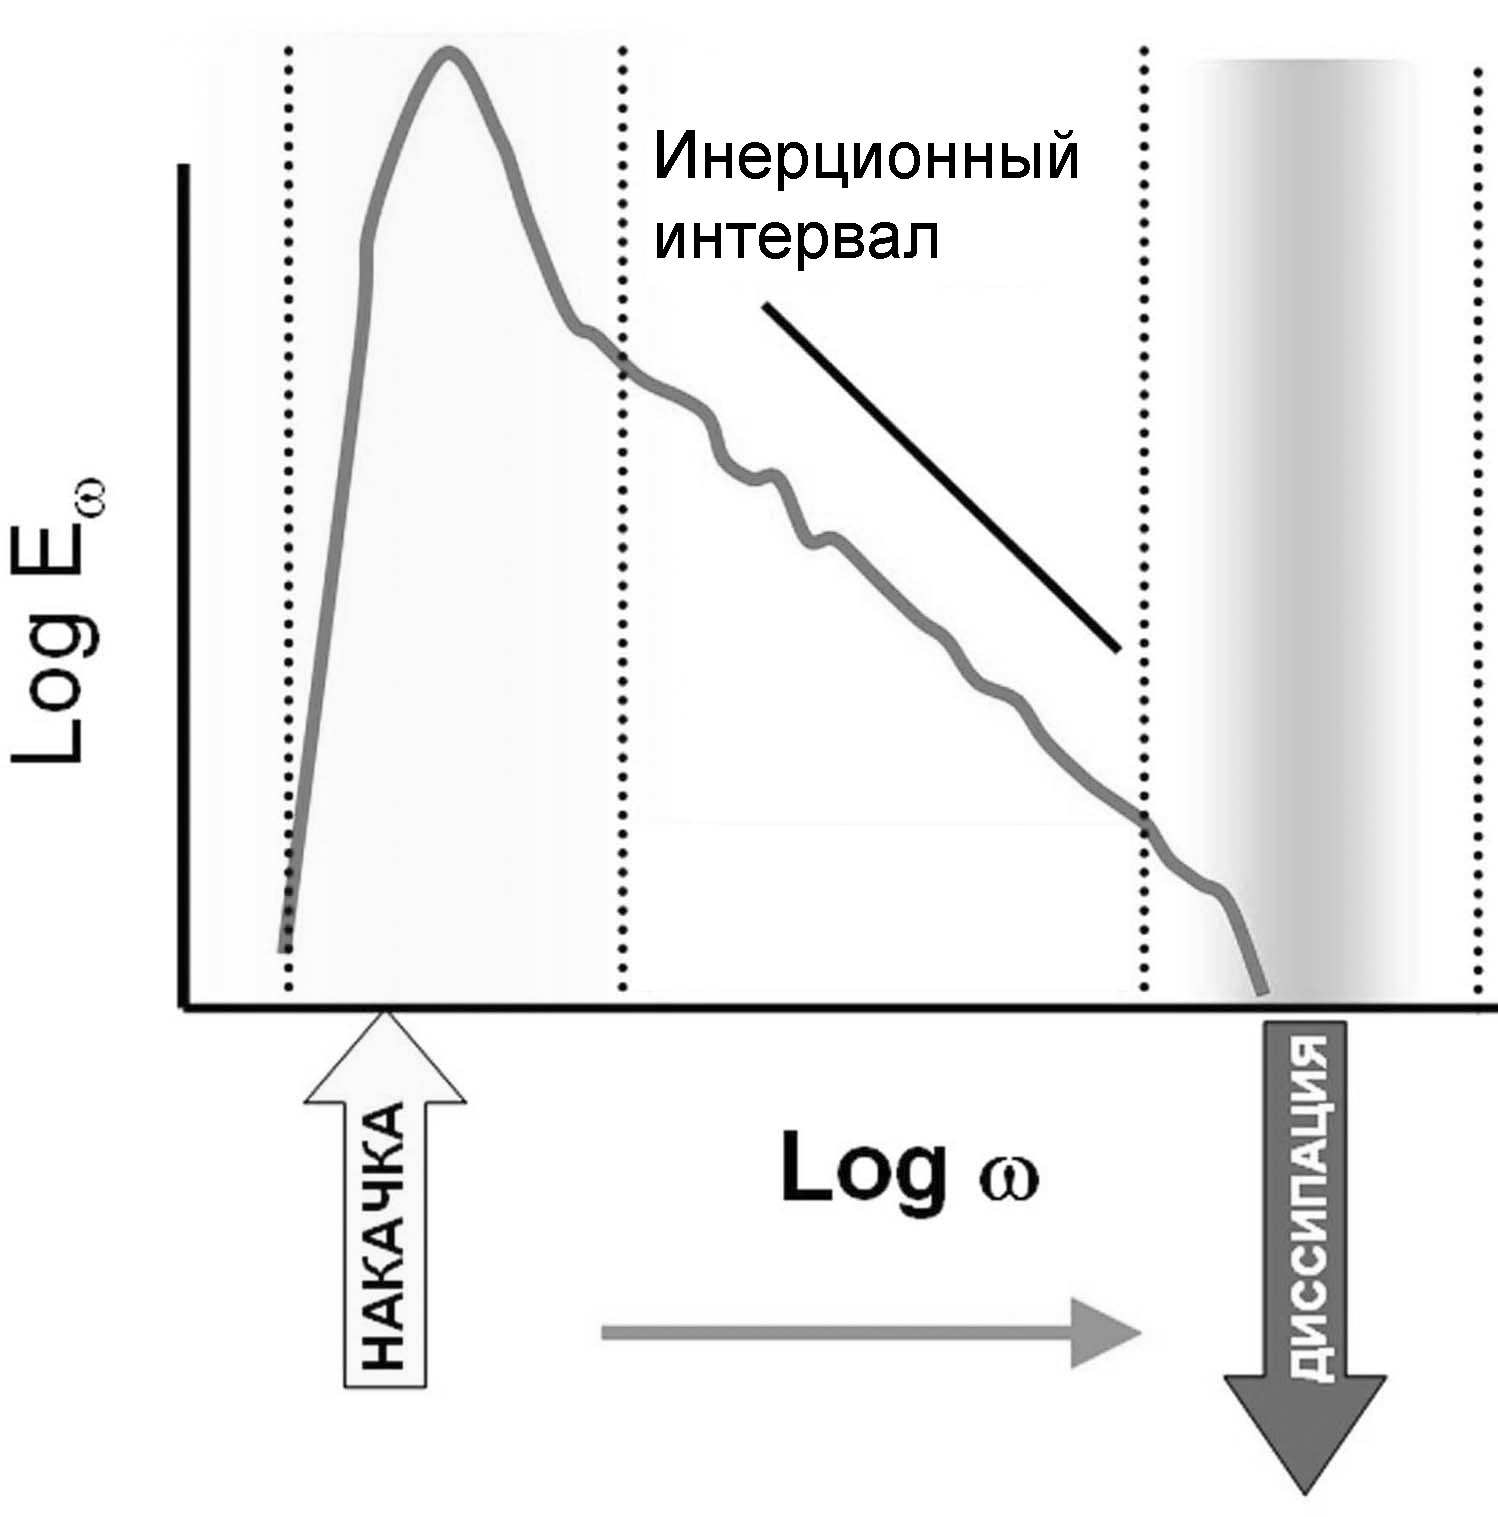
\includegraphics [scale=0.2] {Intro/iner_inter.jpg}
  \caption{} 
  \label{img:turb}  
\end{figure}

Одним из ярких примеров волновой турбулентности являются ветровые волны на поверхности океана.

Ветер, дующий вдоль поверхности изначально гладкой воды, осуществляет накачку энергии в систему волн из-за неустойчивости Кельвина-Гельмгольца \cite[c. 99]{NonLinearWaves}. При этом масштаб накачки составляет порядка одного сантиметра. В результате нелинейного взаимодействия образуются волны других масштабов и энергия передается как в сторону коротких волн, так и в сторону длинных. Через некоторое время на поверхности волны могут образоваться большие волны с характерной длиной волны десятки или сотни метров. И безусловно такие волны уже могут вызывать большие проблемы для кораблей находящихся в это время в море. 
	Обратим внимание, что в стационарном турбулентном каскаде в системе волн осуществляется баланс энергии: сколько энергии приходит из-за взаимодействия волн-ветра, столько же и диссипирует в результате вязкого трения. Однако диссипация эффективно происходит только на коротких масштабах. Т.е. прямой каскад в волновой системе обеспечивает диссипацию энергии приходящей от внешнего источника. %Т.е. можно сказать, что прямой каскад ограничивает величину волн в океане, и не будь этого механизма диссипации водные просторы нашей планеты вряд ли были бы пригодны для мореходства в том виде, к котором мы его знаем.


\section{Закон дисперсии волн на поверхности жидкости}% \label{subsect1_disper}

Волны на поверхности жидкости формируются за счет силы гравитации и сил поверхностного натяжения, причем влияние гравитации преобладает при больших длинах волн, а капиллярных сил - при малых, что видно из закона дисперсии для поверхностных волн, однозначно связывающего угловую частоту волны $\omega$ и модуль волнового вектора $\mathbf{k}$ волн на свободной поверхности жидкости:
\begin{equation}
 \label{eq:disper_dip}
\omega^2 = (gk + \sigma/\rho k^3)th(kh),
\end{equation}
где $g$ - ускорение свободного падения, $\sigma$ - коэффициент поверхностного натяжения, $\rho$ - плотность жидкости, $h$ - глубина жидкости.

В случае, когда $k \gg (g\rho/\sigma)^{1/2}$ влияние гравитационных сил становится пренебрежимо малым по сравнению 
с капиллярными силами. Такие волны называют капиллярными. Волновые вектора $k \ll (g\rho/\sigma)^{1/2}$ соответствуют гравитационному участку закона дисперсии. В промежуточном случае $k \sim (g\rho/\sigma)^{1/2}$ говорят о капиллярно-гравитационных волнах. Для свободной поверхности воды частота соответствующая волновому вектору $k = (g\rho/\sigma)^{1/2}$ перехода от гравитационных волн к капиллярным составляет $\sim$ 17 Гц, при этом длина волны равна $\lambda = 2\pi/k \approx$ 1.5 см. Для поверхности жидкого водорода эта частота также равна $\sim$ 17 Гц, что соответствует длине волны $\sim$ 1.1 см.


Так как плотность жидкого водорода в 13 раз ниже плотности воды, то для возбуждения волн той же амплитуды на поверхности жидкого водорода требуются куда меньшие силы, чем для воды. Инжектирую заряды в объем жидкового водорода можно зарядить его поверхность. Таким образом можно возбуждать волны воздействую электрическим полем непосредственно на заряженную поверхность, что приводят к уникальной возможности экспериментального изучения слабой волновой турбулентности. Использование жидкого водорода в экспериментах по волновой турбулентности уже помогло исследовать явления предсказанные теорией, например стационарный спектр Захарова-Колмогорова в капиллярной турбулентности в широком диапазоне частот \cite{Brazhnikov2001}, а также наблюдать новые явления, которые были успешно объяснены в рамках  приближения слабой турбулентности: например квазиадиабатический распад капиллярной турбулентности \cite{quasiadiabatic} и подавление высокочастотных турбулентных колебаний добавлением низкочастотной возбуждающей силы \cite{addLowFreq}.

Стоит отметить, что если глубина жидкости больше, чем характерная длина волны, то $kh > 2\pi$ и $th(kh)$ можно считать равным 1. Таким образом, в приближении глубокой воды дисперсия гравитационно-капиллярных волн записывается как:


\begin{equation}
 \label{eq:disper}
\omega^2 = gk + \sigma/\rho k^3,
\end{equation}


В экспериментах с гравитационными волнами глубина жидкости была около $ h \approx 7$ см, минимальный волной вектор $k \approx 0.36$ см$^{-1}$, соответственно $th(kh) \approx 0.99$, т.е. влиянием глубины можно пренебречь.


В области высоких частот, где можно пренебречь влиянием гравитационных сил, закон дисперсии будет капиллярным:
\begin{equation}
 \label{eq:disperCap}
\omega^2 = \sigma/\rho k^3
\end{equation}

%В экспериментах с гравитационными волнами глубина жидкости была около $ h \sim 7$ см, минимальный волной вектор $k = 0.36$, соответсвенно $th(kh) \sim 0.99$, т.е. влиянием глубины можно также пренебречь. Таким образом закон дисперсии будет:
%\begin{equation}
% \label{eq:disperGrav}
%\omega^2 = gk,
%\end{equation}

\section{Законы сохранения энергии и импульса} %\label{subsect1_lawSave}

%Из \cite{Brazhnikov2001}. ""Известно, что капиллярные волны на поверхности жидкости характерезуются относительно сильным взаимодействием[?]. Ансамбль взаимодействующих волн может быть описан в рамках кинетического уравнения, вполне аналогичного уравнению Больцмана газовой динамики. Закон дисперсии капиллярных волн является распадным, следовательно, основной вклад во взаимодествие волн вносит трехволновые процессы - распад волны на две с сохранением суммарного волнового вектора и суммарной частоты, а так же обратны ему процесс слияния двух волн в одну.
При взаимодействии волн должны выполняться законы сохранения энергии и импульса. Для капиллярных волн трехволновые процессы могут удовлетворять законам сохранения импульса и энергии, поэтому закон дисперсии в капиллярной область называют распадным. Законы сохранения энергии и импульса для трехволнового процесса:
\begin{equation}
 \label{eq:saveOmega}
\omega_1 = \omega_2 \pm \omega_3
\end{equation}
\begin{equation}
 \label{eq:saveK}
\mbox{\boldmath$k_1$} = \mbox{\boldmath$k_2$} \pm \mbox{\boldmath$k_3$}
\end{equation}

Таким образом при возбуждении на поверхности жидкости волн в области низких частот может быть сформировано турбулентное состояние, в котором поток энергии направлен от области низких частот(область накачки) в сторону больших частот. Теория слабой волновой турбулентности \cite{Zakharov} предсказывает, что основной вклад в перенос энергии по турбулентному капиллярному каскаду вносят как раз трехволновые процессы слияния волн. 

Стоит также отметить, что для гравитационных волн трехволновые процессы запрещены из-за того, что не удовлетворяют законам сохранения энергии и импульса.


\section{Инерционный интервал турбулентного каскада}% \label{subsect1_1_3}

Как было сказано выше характерной особенностью турбулентного каскада является наличие инерционного интервала -  частотного диапазона в котором энергия ни приходит в систему, ни диссипирует.
В настоящий момент имеется довольно много теоретических и экспериментальных работ посвященных изучению инерционного интервала турбулентного каскада в различных системах. Теория слабой волновой турбулентности предсказывает степенное распределение энергии по шкале частот \cite{Zakharov}:
\begin{equation}
\label{eq:EOmega}
E_\omega \sim \omega^{-\alpha}
\end{equation}

С экспериментальной точки зрения удобно исследовать не распределение энергии по волновым векторам(или частотам) напрямую, а парную корреляционную функцию отклонения поверхности от положения равновесия $I(\tau)=<\eta(r, t+\tau)\eta(r,t)>$, так как величину отклонения поверхности от положения равновесия, в отличии от энергии, можно непосредственно экспериментально измерить. Фурье образ парной корреляционной функции отклонения поверхности от равновесного состояния связан с распределением энергии по частотам:
\begin{equation}
\label{eq:EOmegaI}
I_\omega \sim E_\omega \omega^{-4/3} = n(\omega) \omega^{-1/3},
\end{equation}
где $n(\omega)$ - функция распределения капиллярных волн.

Таким образом предсказывается степенная зависимость $I_\omega \sim \omega^{-m}$

В зависимости от характера накачки теория волновой турбулентности предсказывает различные показатели $m$. Для широкополосной накачки (когда ширина полосы накачки сопоставима или больше самой частоты накачки), предсказывается $m$ = 17/6. При накачке узкополосным сигналом в спектре появляются равноудаленные пики, максимумы которых убывают c ростом частоты с показателем $m$ = 23/6. Данные предсказания подтверждаются с помощью компьютерного моделирования \cite{Babiano1995, Babiano1987, Falcovich1988, Pushkarev1996}, так в экспериментальных исследованиях \cite{Brazhnikov_liq_hydr, Falcon2007}. Форма инерционного интервала хорошо экспериментально изучена в спектрах турбулентных каскадов в системе волн на поверхности воды \cite{BrazhnikovWater}, жидкого водорода \cite{Brazhnikov2001}, жидкого гелия \cite{Abdurakhimov2007}, ртути \cite{Falcon2007}.

Стоит отметить, что одной из сложностью для экспериментального исследования и проведения вычислительных экспериментов по исследования турбулентных каскадов является степенное уменьшения энергии волны с ростом частоты. Так как величина показателя степени $m$ находится в районе 2-3, а диапазон частот в котором существует турбулентный каскад может достигать нескольких декад, то для экспериментального исследования поведения турбулентной системы в достаточно широком диапазоне частот, необходимым для наблюдения развитого турбулентного каскада, требуется экспериментальное оборудование обладающее большим динамическим диапазоном. Таким образом экспериментальное исследование инерционного интервала и диссипативной области турбулентных каскадов было практически невозможно до появления широко распространенных АЦП с высоким динамическим диапазоном и достаточной высокой частотой оцифровки, а также развитием компьютерной техники для обработки полученных сигналов.

\section{Положение высокочастотной границы инерционного интервала}% \label{subsect_boundary}

Для определения частотной области, где заканчивается инерционный интервал и начинается диссипация энергии рассмотрим такие важные характеристики волновой системы как вязкое время и нелинейное время.

Вязкое время определяется как характерное время вязкого затухания волны с заданной частотой \cite[стр. 135]{land}.
\begin{equation}
\label{eq:tauNu}
1/\tau_\nu = 2\nu k^2 = 2 \nu \omega^{4/3}(\sigma/\rho)^{2/3},
\end{equation}
где $\nu$ - кинематическая вязкость жидкости.
То есть вязкое время уменьшается с ростом частоты, а следовательно и диссипация энергии на более высоких частотах сильнее.


Характерное время нелинейного взаимодействия капиллярных волн можно выразить через параметры жидкости и функцию распределения капиллярных волн $n(\omega)$:
\begin{equation}
\label{eq:tauNl}
1/\tau_{nl} = |V_\omega|^2 n(\omega)
\end{equation}

Где $V(\omega) \approx (\sigma/\rho^{3/2})\omega^{3/2}$ - коэффициент трехволнового нелинейного взаимодействия капиллярных волн.

%Функцию распределения капиллярных волн $n(\omega) \sim E_{\omega}\omega^{-1}$ 
В развитом турбулентном каскаде энергия передается от низких частот к высоким практически без потерь до тех пор, пока скорость диссипации не становится сравнима с потом энергии. Таким образом положение высокочастотной границы инерционного интервала можно определить как частоту, на которой совпадают времена вязкого затухания и нелинейного взаимодействия волн.

Из уравнений (\ref{eq:EOmegaI}, \ref{eq:tauNu}, \ref{eq:tauNl}), используя известные значения $m$ = 17/6 для широкополосной накачки и $m$ = 23/6 для монохроматической накачки, получаем оценку амплитудной зависимости частоты границы инерционного интервала $\omega_b \sim \eta_p^{2.4}$ для широкополосной накачки и $\omega_b \sim \eta_p^{4/3}$ для узкополосной накачки. Несмотря на то, что отдельные экспериментальные работы по измерению поведения положения границы инерционного интервала производились \cite{Brazhnikov_bound_freq}, работ направленных на создание общей картины поведения положения границы инерционного интервала для разных типов накачки и разной геометрии экспериментальной ячейки не было.
%хренности $\Omega_0$ в случае стоячих волн определяется как:

\section{Диссипативная область турбулентного каскада}% \label{subsect_disp}

На частотах больших граничной частоты инерционного интервала $\omega_b$ спектр зависит и от специфики затухания, и от нелинейного взаимодействия. Несмотря на то, что в диссипативной области вязкое время превышает нелинейное и преобладают процессы затухания, нелинейные процессы существенно влияют на форму спектра. Если волны в диссипативном интервале взаимодействуют в основном с ближайшими соседями, а не с волнами из инерционного интервала, то распределение энергии по волнам в области диссипации становиться близким к экспоненциальному.
Если же волны в диссипативной области $\omega \gg \omega_b$ взаимодействует волнами из инерционного интервала $\omega \ll \omega_b$, то распределение энергии по волнам несколько отличается от экспоненциального. Детальное рассмотрение дает “квазипланковский” спектр корреляционной функции в диссипативной области  \cite{Ryzhenkova1990}
\begin{equation}
% \label{eq:tauNu}
<\eta_\omega^2> \sim \omega^{-s} e^{-\omega/\omega_d},
\end{equation}			
где s - некая константа. Численные вычисления для дискретного кинетического уравнения \cite{Ryzhenkova1990} подтверждают экспоненциальную зависимость волнового числа заполнения в области сильного затухания. Величину $\omega_d$ имеющую размерность частоты и отвечающей за то насколько быстро затухает турбулентный спектр в диссипативной области будем называть частотой вязкого затухания диссипативной области.
	
%	Мы представляем первое экспериментальное наблюдение турбулентных спектров капиллярных волн в диссипативной области возбужденных низкочастотной случайной силой на поверхности жидкого водорода.

%
%Слабая волновая теория предсказывает существование стационарного неравновесного состояния в системе взаимодействующих капиллярных волн - спектр Колмогорова-Захарова для спектральной плотности энергии $\varepsilon(k)$ волн в инерционном интервале.
%\begin{equation}
%% \label{eq:tauNu}
% \varepsilon(k) \sim P^{1/2}k^{-7/4}
%\end{equation}
%
\todo{Разобраться с этим.(это нужно на стр. 25, ссылка на формулу(3))}

%Используя соотношение между спектральной плотностью энергии $\varepsilon(k)$ и парной корреляционной функцией высоты поверхности $\eta(\mathbf{r}, t)$, и принимая во внимание закон дисперсии капиллярных волн $\omega(k) \sim k^{3/2}$, можно получить частотный спектр корреляционной функции $<\eta(t+\tau)\eta(t)>$:
%\begin{equation}
% \label{eq:tauNu}
%<\eta_\omega^2> \sim (\sigma k^2)^{-1} \varepsilon(k)(d\omega/dk)^{-1} \sim P^{1/2} \omega^{-17/6}.
%\end{equation}

%Слабая волновая теория предсказывает существование стационарного неравновесного состояния в системе взаимодействующих капиллярных волн - спектр Колмогорова-Захарова для спектральной плотности энергии е(к) волн в инерционном интервале.
%$(k)P1/2k-7/4$		(1)
%Используя соотношение между спектральной плотностью энергии и парной корреляционной функцией высоты поверхности (r, t), и принимая во внимание закон дисперсии капиллярных волн (k) k3/2, можно получить частотный спектр корреляционной функции <(t+)(t)>:
%<|2|>(k2)-1(k)(d/dk)-1P1/2-17/6
%	Этот стационарный спектр характеризуется одной величиной P - потоком энергии на большие частоты . На больших частотах передаваемая энергия диссипирует из-за вязких потерь и турбулентный каскад разрушается. Следовательно для поддержания распределения (2) или (1) постоянным во времени, система должна постоянно накачиваться энергией на низких частотах. Высокочастотная граница инерционного интервала d, где распределение (2) еще остается верным, может быть оценена из предположения, что время вязкого затухания () и время нелинейного взаимодействия nl() равны по порядку для волн на частоте d. Это предположение дает нам [5]:
%<........>  (3)





%Экспоненциальное падение в турбулентном каскаде на частотах выше $\omega_b$ наблюдали в системе капиллярно-гравитационных волн на поверхности жидкого водорода и гелия [12, 13]. В экспериментах с жидким водородом [12] в случае широкополосной накачки было показано, что характерная частота $f_d$ растет с увеличением амплитуды возбуждающей силы по степенному закону $f_d \sim A^{0.85}$.

Экспериментальные ячейки имеют конечные размеры, поэтому спектр поверхностных возбуждений носит дискретный характер. Это накладывает дополнительные ограничения на выполнение законов сохранения энергии и импульса \cite{Kartashova1991}. В экспериментальных работах \cite{Brazhnikov2014, Aburakhimov2015} было показано, что выбором размеров ячейки при накачке на некоторых частотах можно организовать передачу энергии как на высокие, так и на низкие частоты.
Одной из целей настоящей работы было проведение подробных исследований зависимостей высокочастотного края инерционного интервала $\omega_b$ и характерной частоты $\omega_d$ от амплитуды возбуждающей силы на поверхности воды в цилиндрической и квадратной ячейках при амплитудах накачки меньше порогового значения, при котором возникает параметрическая неустойчивость Фарадея.

\section{Разрешенные моды в ограниченной геометрии} %\label{subsect1_geometr}
%геометрия волн в зависимости от геомертрии ячейки
Рисунок волн на поверхности сильно зависит от геометрии сосуда и способа возбуждения волн.
В случае, если длина затухания волны много больше характерного размера ячейки, при возбуждении волн на поверхности жидкости возникнет система стоячих волн. Форма стоячих волн будет зависеть от граничных условий и возбуждаемой моды. Граничным условием для волн в ограниченной ячейке является неспособность воды проходить через стенку ячейки, т.е. нормальная (к стенке ячейки) компонента скорости жидкости должна быть равна нулю. Так для цилиндрической ячейки радиуса $r_0$ резонансные моды волн будут описываться функцией Бесселя:

\begin{equation}
 \label{eq:Bessel}
h(r, \phi, t) = A J_0(k_nr) cos(\phi m) cos(\omega t),
\end{equation}
причем $k_n$ должна удовлетворять требованию ${J_0}'(k_nr_0) = 0$. Иными словами на границе ячейки должна быть пучность стоячей волны.

Если $m$ = 0, то мода будет радиальной, в таком случае скаляр $k$ играет роль волнового числа: при больших значениях $R/\lambda$, ($\lambda = 2\pi/k$ – длина возбуждаемой волны) и на большом расстоянии $r \gg \lambda$ от центра ячейки в узком угловом секторе цилиндрическую волну можно рассматривать как плоскую волну с волновым числом $k$ в одномерном k-пространстве.

В прямоугольной ячейке стоячие волны описываются суммой двух стоячих перпендикулярных синусоидальных волн:
\begin{equation}
\label{eq:waveStand}
h(x, y, t) = A_1 sin(kx)cos(\omega t)+A_2 sin(ky)cos(\omega t+ \phi)
\end{equation}
где $\phi$ разность фаз между стоячими волнами в разных направлениях.

Бегущие волны, распространяющиеся от двух перпендикулярных стенок прямоугольной ячейки будут задаваться выражением:
\begin{equation}
\label{eq:waveRun}
h(x, y, t) = A_1 sin(kx-\omega t)+A_2 sin(ky-\omega t+ \phi)
\end{equation}



%\section{Возбуждение волн в ячейке вертикальной тряской} %\label{subsect_boundary}

%Турбулентность в системе волн наряду с вихревой турбулентностью играет значительную роль во многих процессах, происходящих на Земле и во Вселенной. Она является объектом интенсивных исследований во многих системах: на поверхности океана, в атмосфере, в плазме [1]. 
%Турбулентноcть на поверхности воды в гравитационно-капиллярном интервале частот изучалась многими исследователями в течение нескольких последних десятилетий [2–5]. Для возбуждения волн использовали различные методики. Так, в [2] применяли специальные лопатки (мешалки), погруженные в жидкость. Однако в большинстве работ для генерации волн используют параметрическую неустойчивость поверхности жидкости, совершающей вынужденные вертикальные колебания с ускорениями выше некоторого порогового значения (неустойчивость Фарадея) [3–5]. Отличительной чертой этой методики является высокий уровень возбуждения волн сразу после возникновения неустойчивости на поверхности. Такая особенность методики возбуждения не позволяет работать с волнами малой амплитуды. Кроме того, как выяснилось, при сильном возбуждении наряду с нелинейным взаимодействием волн наблюдается генерация вихревого движения [6, 7]. Недавно в [8, 9] было показано, что завихренность формируется в результате взаимодействия нелинейных волн, имеющих непараллельные волновые векторы, т.е. в двумерном пространстве волновых векторов k. В [10] волны на поверхности цилиндрической ячейки возбуждали с помощью кольца, касающегося поверхности воды вблизи стенок ячейки. На поверхности возбуждалась только радиальная мода. В этом случае стоячие волны на поверхности описываются функцией Бесселя параметра $Rk$ ($R$ – радиус ячейки). Скаляр $k$ играет роль волнового числа: при больших значениях $R/\lambda$, ($\lambda = 2*\pi/k$ – длина возбуждаемой волны) и на большом расстоянии $r \gg \lambda$ от центра ячейки в узком угловом секторе цилиндрическую волну можно рассматривать как плоскую волну с волновым числом k в одномерном k-пространстве. Экспериментальные результаты [10] оказались в хорошем согласии с теорией слабой (волновой) турбулентности [1].

%В настоящем сообщении представлены экспериментальные результаты исследований турбулентности в системе волн на поверхности воды, возбуждаемых вертикальными колебаниями ячейки за счет краевого эффекта смачивания при ускорениях меньше порового значения возникновения неустойчивости Фарадея в цилиндрической ячейке, когда вихревое движение еще не наблюдается, и в квадратной ячейке, где вихревое движение при этих уровнях накачки хорошо развито.

%=======
\section{Способы возбуждения волн на поверхности жидкости}\label{p1_methodsExt}

%Турбулентность в системе волн наряду с вихревой турбулентностью играет значительную роль во многих процессах, происходящих на Земле и во Вселенной. Она является объектом интенсивных исследований во многих системах: на поверхности океана, в атмосфере, в плазме [1]. 
Турбулентноcть на поверхности воды в гравитационно-капиллярном интервале частот изучалась многими исследователями в течение нескольких последних десятилетий \cite{Falcon2007, Henry2000, Shats2010, Denissenko2007}. В лабораторных условиях волны на поверхности жидкости могут возбуждаться различными способами: при помощи волнопродукторов \cite{Havelock1929, Falcon2007}, электрическими силами, действующими на границу раздела жидкостей с разной диэлектрической проницаемостью \cite{Kalinichenko1982} или на поверхность заряженной жидкости \cite{Brazhnikov2002}, колебаниями сосуда с жидкостью в вертикальном направлении как целого \cite{Miles1990}.

В последнем случае возможны два механизма возбуждения волн на поверхности воды. Первый осуществляется благодаря наличию мениска на границе ячейки. При вертикальных колебаниях равновесный радиус мениска меняется в зависимости от величины вертикального ускорения, что приводит к появлению на поверхности жидкости волн с частотой равной частоте вертикальных колебаний ячейки. 

Второй способ возникновения волн - в результате развития пороговой параметрической неустойчивости на поверхности жидкости впервые описанной Фарадеем \cite{Faraday1831}. Так как неустойчивость параметрическая, то частота возбужденных волн в два раза меньше частоты вертикальных колебаний ячейки. Во многих работах для генерации волн используют эту параметрическую неустойчивость Фарадея поверхности жидкости \cite{Henry2000, Shats2010, Denissenko2007}. Отличительной чертой этой методики является высокий уровень возбуждения волн сразу после возникновения неустойчивости на поверхности. Однако такая особенность методики возбуждения не позволяет работать с волнами относительно малой амплитуды.

При вертикальных колебаниях сосуда с жидкостью относительно низкой амплитуды параметрическая неустойчивость Фарадея не возникает, так как является пороговым эффектом. Поэтому для наблюдения спектров турбулентного каскада на поверхности воды использовалось возбуждение волн с помощью вертикальных колебаний с амплитудой ниже порога параметрической неустойчивости. 

Стоит отметить, что при возбуждении волн на поверхности воды с помощью мениска в цилиндрической ячейки возбуждаются только радиальные моды, а при развитии параметрической неустойчивости происходит возбуждение и азимутальной моды.



При наблюдении волновой турбулентности на поверхности жидкого водорода удобнее использовать возбуждение волн с помощью электрического поля. В этом случае амплитуда волн ограничивается напряжением пробоя и размерами оптического окна криостата, через которое с помощью лазерного луча производится регистрация волн \cite{Brazhnikov2002}.


\section{Метод детектирования волн на поверхности жидкости}\label{p1_methodDetect}

Существует много методик регистрации капиллярных волн. Можно регистрировать волны на поверхности жидкости с помощью преломленного или отраженного лазерного луча от сравнительно небольшого участка поверхности жидкости \cite{Brazhnikov_IET}. Для регистрации волн на поверхности проводящей жидкости в работе \cite{Falcon2007} в жидкость вводили вертикально ориентированный отрезок изолированной металлической проволоки. В результате образуется цилиндрический конденсатор, одной из обкладок которого служит поверхность проволоки, а другой – проводящая жидкость. По изменению емкости конденсатора со временем можно судить о колебаниях уровня жидкости в точке контакта изолированной проволоки и жидкости.
В работе \cite{Wright1996, Henry2000} камерой регистрировали свет прошедший через полупрозрачную жидкость, а для обеспечения диффузного распространения света в объеме жидкости в рабочую ячейку с жидкостью (водой) вводили полистироловые шарики диаметром 1 мкм или добавляли обычное молоко. На фотографии колеблющейся поверхности яркость отдельных точек определяется высотой уровня поверхности жидкости, т.е. по распределению яркости точек на поверхности можно судить о распределении энергии (амплитуде колебаний) по волновым векторам на поверхности освещаемой снизу "мутной"  жидкости. В работе \cite{Fujimura2008} возбуждение и регистрация колебаний на поверхности воды производится с помощью электрического поля емкостным методом. Для этого на стенке прямоугольной кварцевой кюветы помещены полоски из алюминия, которые играют роль конденсатора.

Остановимся подробнее на методики измерения волн с помощью отраженного лазерного луча.

\begin{figure}[ht] 
  \center
  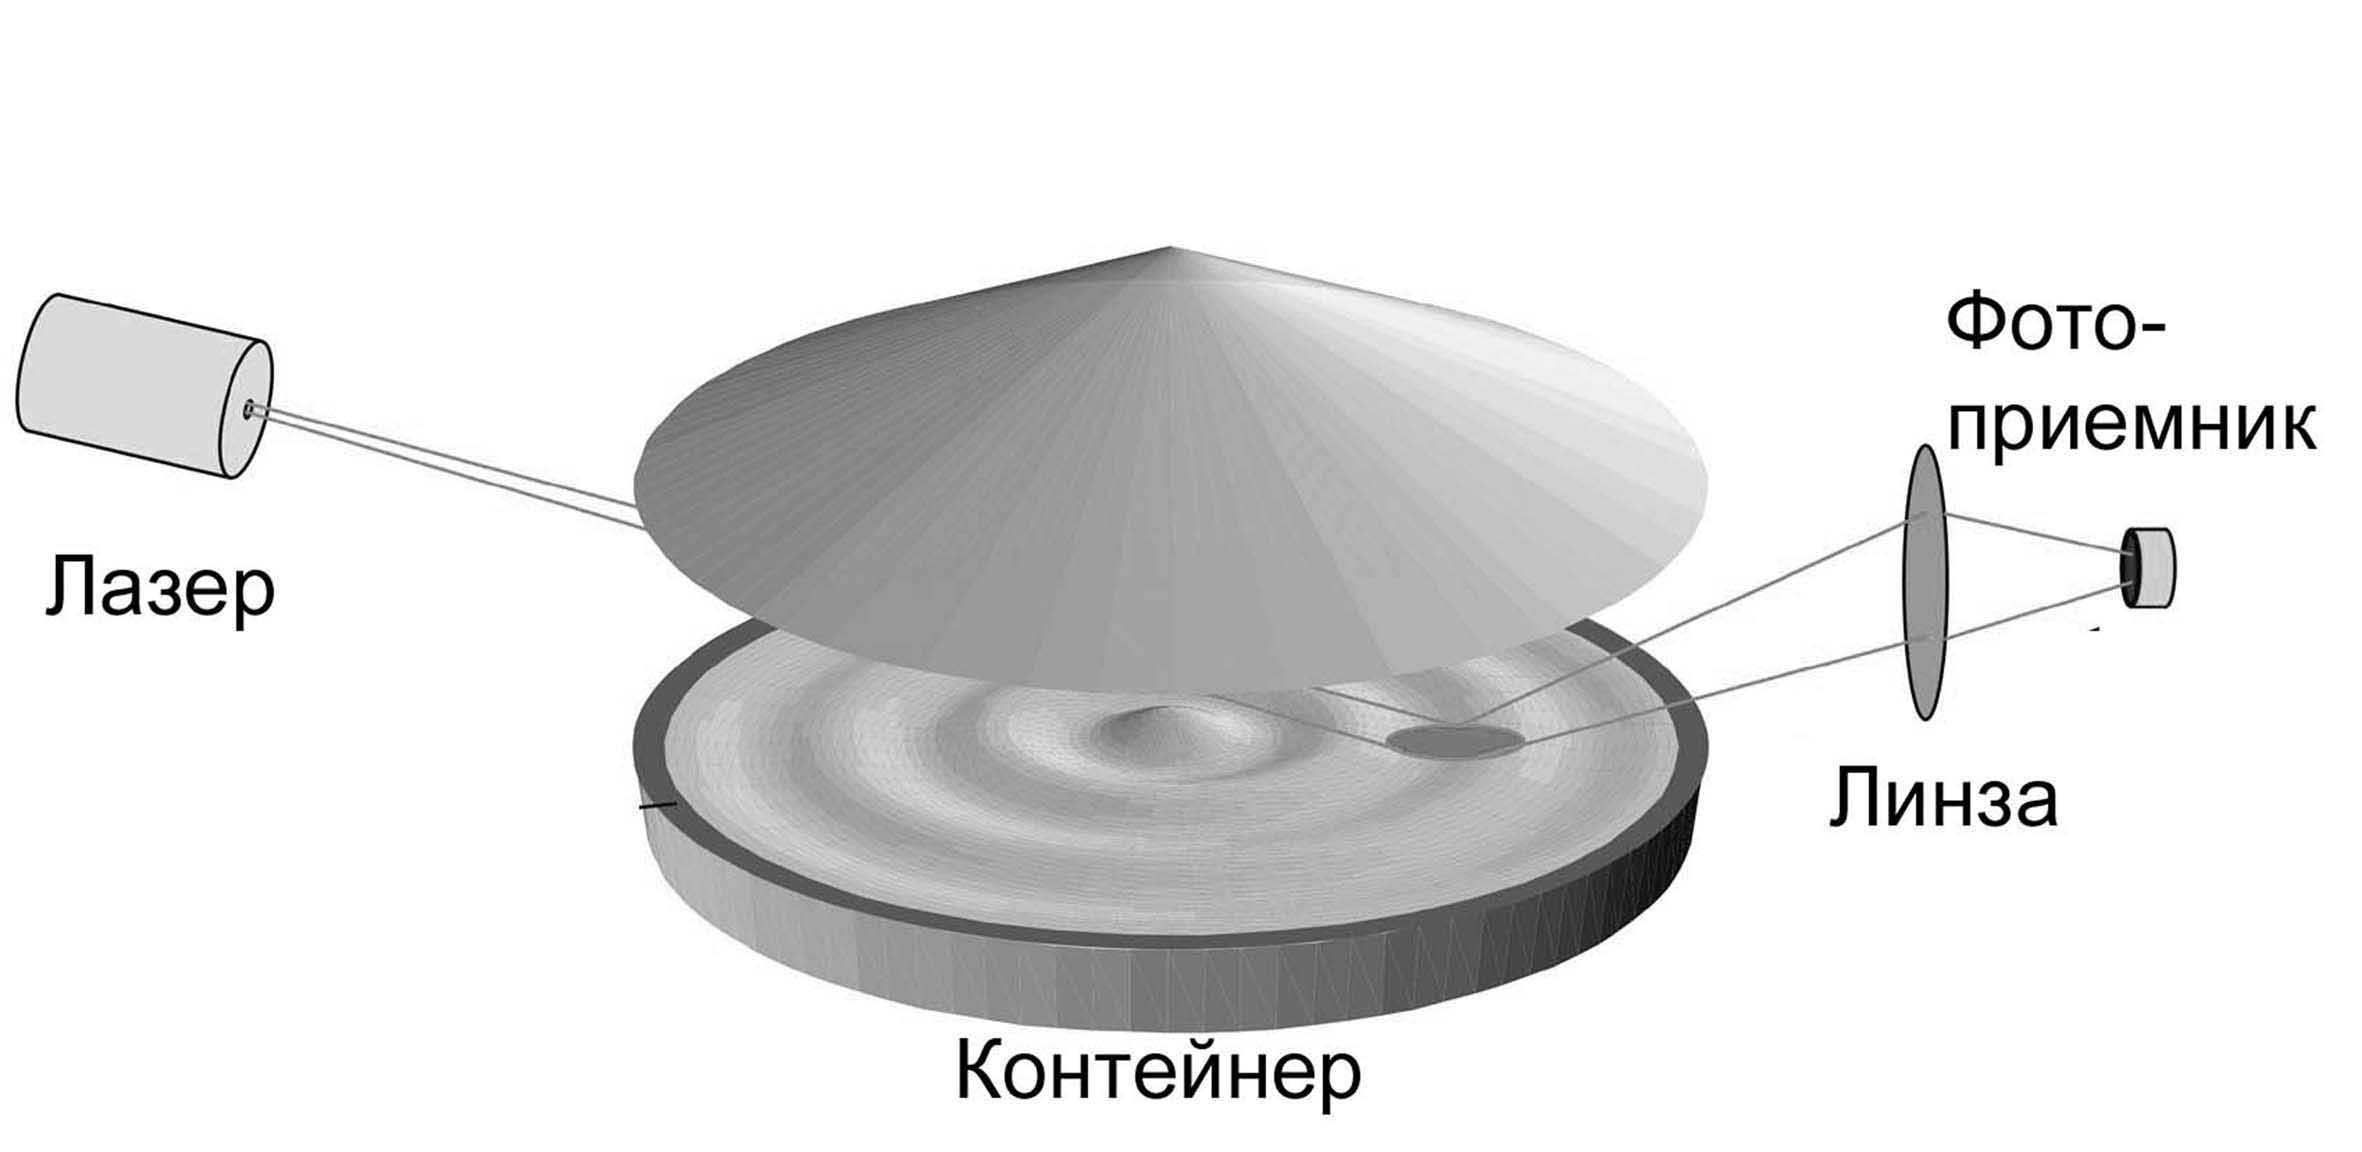
\includegraphics [scale=0.15] {Intro/laser.jpg}
  \caption{Схема методики измерения волн на поверхности жидкости с помощью отраженного лазерного луча.} 
  \label{img:laser}
\end{figure}

Колебания поверхности детектируются по схеме, показанной на рисунке \ref{img:laser}. Лазерный луч, отраженный от поверхности жидкого водорода, фокусируется линзой на фотоприемник. Угол скольжения лазерного луча (угол между лазерным лучом и плоскостью поверхности жидкости) к поверхности жидкого водорода составляет примерно 0.2 рад. Максимальный угол отклонения поверхности жидкости составляет 0.05 рад.

В зависимости от характерного размера $a$ пятна лазерного луча на поверхности жидкости и длины волны $\lambda$ детектируемого колебания возможны два метода обработки сигнала с фотоприемника:

1. $ a \ll \lambda$. «Узкий луч». Характерный размер пятна лазерного луча много меньше длины волны. В этом случае мощность отраженного луча зависит от угла отражения, то есть в приближении малых углов мощность принимаемого сигнала фотоприемника линейно зависит от угла отражения.
\begin{equation}
%\label{eq:waveStand}
P(t) \sim R(\alpha + \phi(t)) \approx R(\alpha) + const \phi(t)
\end{equation}
Для квадрата Фурье-компонент:
\begin{equation}
%\label{eq:waveStand}
P^2_\omega \sim \phi^2_\omega
\end{equation}
где $P(t)$ - мощность сигнала на фотоприемнике, $R$ – коэффициент отражения.

2. $a \gg \lambda$. «Широкий луч». Характерный размер пятна лазерного луча много больше длины волны. В этом случае мощность отраженного луча является интегральной характеристикой поверхности. В результате усреднения получится следующая зависимость \cite{Brazhnikov_IET}:
\begin{equation}
%\label{eq:waveStand}
P^2_\omega \sim I_\omega
\end{equation}

\section{Возбуждение вихревых течений поверхностными волнами}% \label{sect3_1}

%	Сравнительно недавно было обнаружено, что при возбуждении на поверхности жидкости неустойчивости Фарадея помимо волн возбуждаются также вихревые движения \cite{VonKameke2011, Francois2014}, причем статистические характеристики этого движения описываются схожими соотношениями, что и статистика двумерной турбулентности, несмотря на то, что движение жидкости существенно трехмерно.
	Вихревые системы уже давно и прочно ассоциируются с непредсказуемым турбулентным движение. Иногда турбулентное вихревое состояние возникает из спокойного, нетурбулентного состояния, например при обтекании препятствия ламинарным потоком может возникнуть вихревой след сложной структуры, так называемая дорожка Кармана.

Сравнительно недавно было обнаружено, что при параметрическом возбуждении колебаний наряду с волновым движением на поверхности жидкости также наблюдается течение, демонстрирующее хаотическое поведение \cite{Ramshankar1990}. Впоследствии было показано, что это течение соленоидально и с увеличением амплитуды волн может оказаться достаточно интенсивным для формирования турбулентного каскада \cite{VonKameke2011, Francois2014, Francois2013} подобно обратному каскаду в двумерной турбулентности \cite{Kraichnan1967}. Несмотря на большое количество экспериментальных исследований, посвященных волнам Фарадея, природа возникновения в них течения до настоящего времени не выяснена. В работе \cite{Mesquita1992} это течение пытались описать как средний дрейф Стокса \cite{Stokes1847} для случайного волнового поля. Однако найденное в эксперименте значение коэффициента диффузии пассивного скаляра почти на порядок превышало теоретическое.	
	Однако интерес к такому вихревое движение не ограничивается интересом к модельному объекта для изучения свойство двумерной турбулентности.
	 Наше исследование показало [F5], что генерация вихревого движения не является особенностью неустойчивости Фарадея, а является следствием нелинейного взаимодействия волн, распространяющихся под углом друг к другу. Таким образом данное явление уже имеет отношение к движению поверхности океана. В частности оно может играть значительную роль в перемешивании планктона и движению загрязняющих веществ на поверхности воды \cite{Falkovich2009}.
	Еще, стоит отметить, что изучив механизм генерации вихревых течений поверхностными волнами можно научиться создавать вихревое движение заданное формы, возбуждая на поверхности рассчитанный волновой пакет.
	
Для количественного изучения вихревых движений используется величина завихренности, определяемая как:

\begin{equation}
 \label{eq:defVort}
\Omega(x, y) = \frac{\partial V_x}{\partial y} - \frac{\partial V_y}{\partial x}
\end{equation}
где $V_x$, $V_y$ – компоненты скорости жидкости. 



В данной работе будет предложен механизм нелинейной генерации вихревого движения волнами на поверхности жидкости, а так же представлены результаты экспериментов, которые демонстрируют, что формирование вихревого движения не является специфической чертой волн Фарадея, а связано с двухмерностью волнового движения на поверхности жидкости.



%Кроме того, как выяснилось, при сильном возбуждении наряду с нелинейным взаимодействием волн наблюдается генерация вихревого движения \cite{Shats2005, VonKameke2011}.
% Недавно в [F5, F6] было показано, что завихренность формируется в результате взаимодействия нелинейных волн, имеющих непараллельные волновые векторы, т.е. в двумерном пространстве волновых векторов k. В \cite{Brazhnikov_liq_hydr} волны на поверхности цилиндрической ячейки возбуждали с помощью кольца, касающегося поверхности воды вблизи стенок ячейки. На поверхности возбуждалась только радиальная мода. В этом случае стоячие волны на поверхности описываются функцией Бесселя параметра $Rk$ ($R$ – радиус ячейки). Скаляр $k$ играет роль волнового числа: при больших значениях $R/\lambda$, ($\lambda = 2*\pi/k$ – длина возбуждаемой волны) и на большом расстоянии $r \gg \lambda$ от центра ячейки в узком угловом секторе цилиндрическую волну можно рассматривать как плоскую волну с волновым числом k в одномерном k-пространстве. Экспериментальные результаты \cite{Brazhnikov_liq_hydr} оказались в хорошем согласии с теорией слабой (волновой) турбулентности \cite{Zakharov}.

%В настоящем сообщении представлены экспериментальные результаты исследований турбулентности в системе волн на поверхности воды, возбуждаемых вертикальными колебаниями ячейки за счет краевого эффекта смачивания при ускорениях меньше порового значения возникновения неустойчивости Фарадея в цилиндрической ячейке, когда вихревое движение еще не наблюдается, и в квадратной ячейке, где вихревое движение при этих уровнях накачки хорошо развито.
%Гидродинамика жидкости со свободной поверхностью давно является предметом теоретических и экспериментальных исследований. 











%
%
%
%
%
%
%\clearpage